\chapter{Implementação }
% ---
%Neste capitulo visara mostrar os métodos e procedimentos utilizados para implementação da solução do problema evidenciado nos capítulos anteriores .
Neste capítulo será aplicado as técnicas, métodos e procedimentos utilizados para implementação da solução dos problemas evidenciados nos capítulos anteriores.
% ---
\subsection{Códigos da Implementação}

{\color{red} adicionar label e melhorar a descrição}

Nesta parte do código acontece a validação de login do usuário, onde o mesmo se encarrega e enviar os dados informados direto para a API valida-los.
\begin{figure}[H]
	

\centering
\mbox{%
	\subfigure[Tela com a implementação do Login da \textit{Smart Solution}]{\label{LoginCodigo}%
		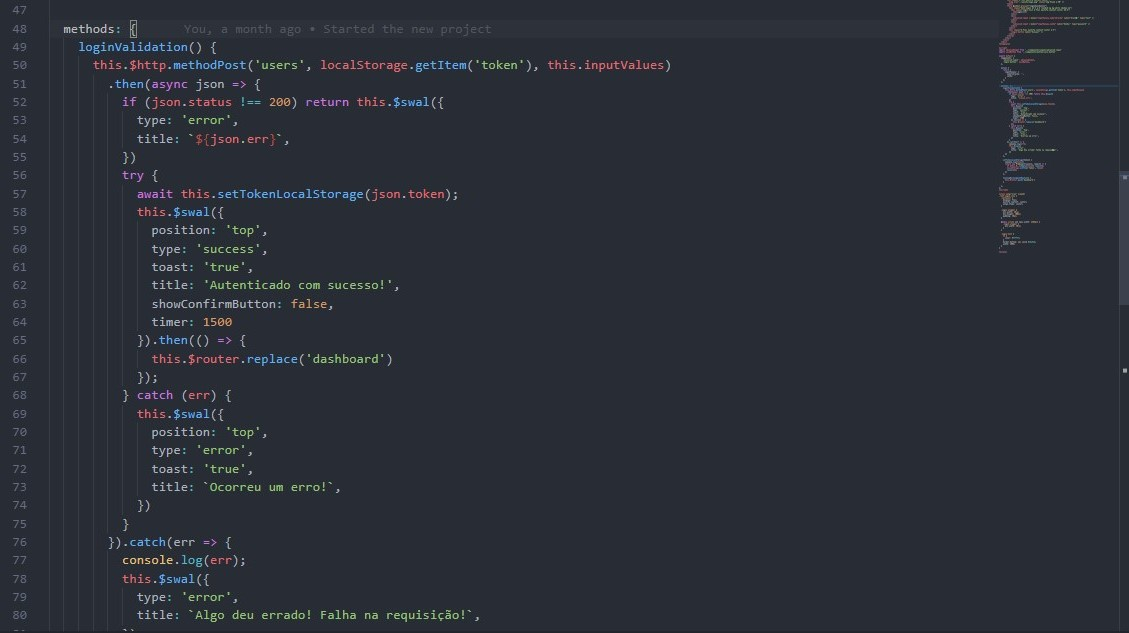
\includegraphics[scale=0.60]{Figuras/LoginCodigo}}
}	
	
	
\end{figure}
\newpage

{\color{red} adicionar label  a Figura X}
Após os dados do usuário serem enviados do APP para a API, neste arquivo a requisição é recebida e enviada para a classe que cuidará das validações.
\begin{figure}[H]
	\centering
	\mbox{%
			\subfigure[Tela de implementação da rota de Login da\textit{Smart Solution}]{\label{Rotalogin}
			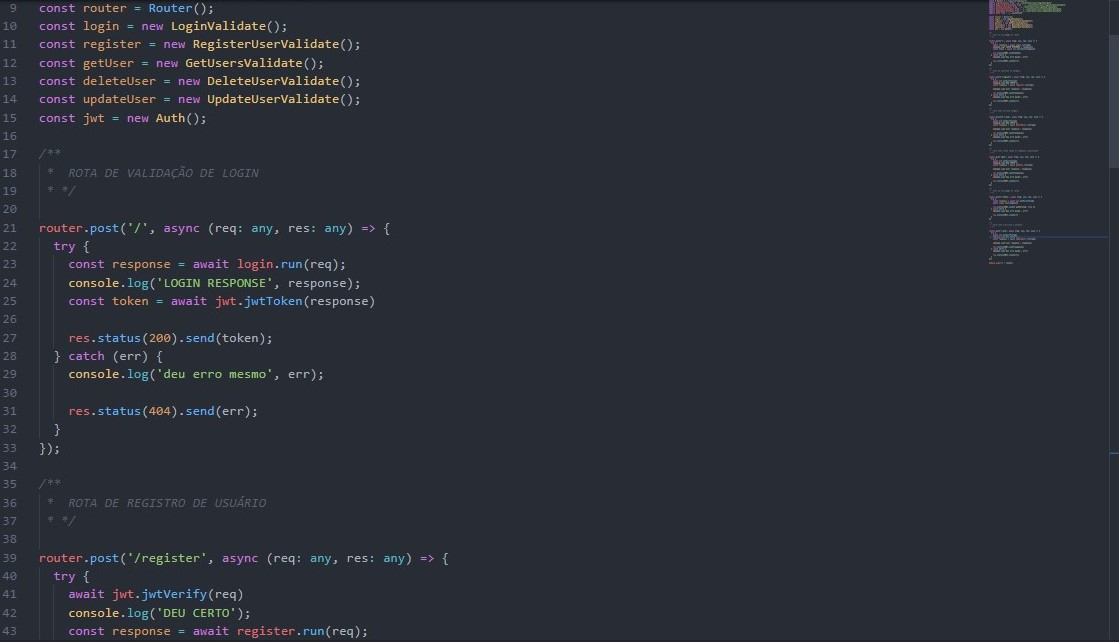
\includegraphics[scale=0.60]{Figuras/Rotalogin}}\qquad
		
	}
	
	
\end{figure}
\newpage
{\color{red} adicionar label  a Figura X}

Chegando na classe de validação, os dados que foram enviados da tela de login são validados, se existe algo na requisição, se os dados enviados existem, caso alguma dessas validações venha a ter erros, API rejeita os dados enviados mandando uma mensagem de erro de volta para o usuário. 

\begin{figure}[H]
	\centering
	\mbox{%
			\subfigure[Tela com a implementação da validação dos dados de Login da\textit{Smart Solution}]{\label{Validacaologin}
			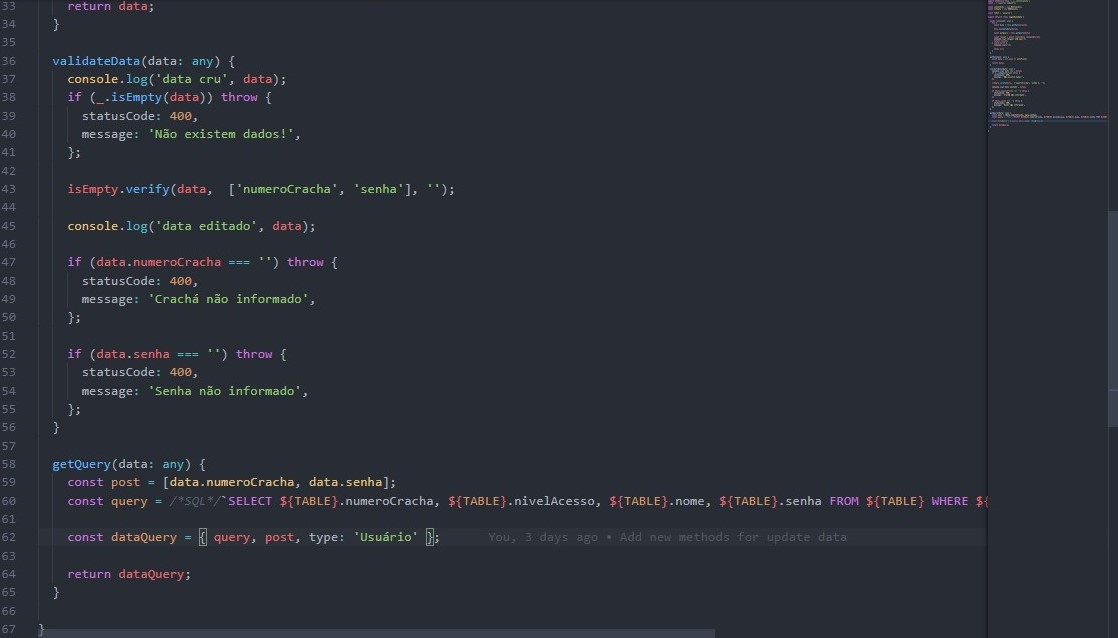
\includegraphics[scale=0.60]{Figuras/Validacaologin}}\qquad
		
	}
	
	
\end{figure}
\newpage
{\color{red} adicionar label  a Figura X}

Por fim, depois de os dados terem sido validados, o mesmo será enviado para a classe que é responsável por se comunicar com o banco de dados, buscando esse usuário no banco de dados, casa a busca retorne um erro é porque esse usuário não existe no banco de dados, caso contrário, o sistema retornará a requisição com o status de sucesso, permitindo assim a entrada do usuário no sistema.
\begin{figure}[H]

	\centering
	\mbox{%
			\subfigure[Tela da implementação com a comunicação para o banco de dados da\textit{Smart Solution}]{\label{DaoLogin}
			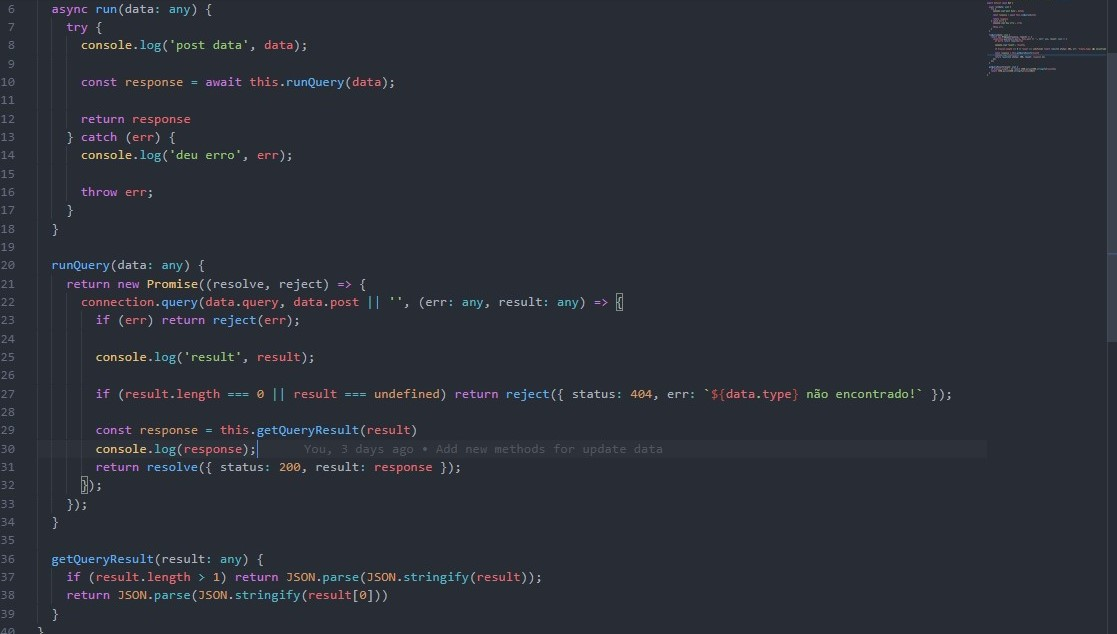
\includegraphics[scale=0.60]{Figuras/DaoLogin}}\qquad
		
	}
	
	
\end{figure}

\section{Desenvolvimento da Aplicação Cliente}
% ---
{\color{red} adicionar label  a Figura X}

Na aplicação Mobile foi usado a tecnologia Vue.js no qual será usado para desenvolver a versão mobile do \textit{Smart Solution}, por ser uma plataforma de desenvolvimento híbrido, possibilitará ser usado tanto no ambiente Android quanto no IOS. Já a aplicação Web será desenvolvida nos próximos semestres e será usado a tecnologia angular por ser semelhante ao Ionic e confiável no desenvolvimento.
% ---

\section{Desenvolvimento da Aplicação Server}
% ---
Para desenvolver a aplicação server, que é responsável pelos endpoints e comunicação com o banco de dados foi utilizado o superconjunto Node.Js, pois essa linguagem facilitará todas as requisições a serem realizadas com dinamismo e agilidade.
% ---
\section{Framework para Conexão Restful}
% ---
A ferramenta para conexão Rest aplicada em conjunto com o Node.Js tanto na API quanto no Client (termo utilizado para definir a versão que o usuário terá interação) possibilita que a comunicação seja feita entre o Client e API e da API para o banco de dados.
% ---
\section{Conexão com Banco de Dados}
% ---
O sistema de gerenciamento banco de dados utilizados foi o MySQL, implementado inicialmente apenas para ambiente de desenvolvimento e teste, permitindo que as vertentes do projeto sejam exploradas de forma livre.
% ---
\newpage
\section{Telas Implementadas}
% ----

{\color{red} adicionar label  as Figuras X e melhorar a introdução}


Tela que permite o usuário entrar no sistema WEB com seu numero de crachá e senha.

\begin{figure}[H]
	\caption{\label{Login_WEB_1}Tela de login}
	\centering
	\mbox{%
		\subfigure[Próprio autor]{\label{Login_WEB_1}%
			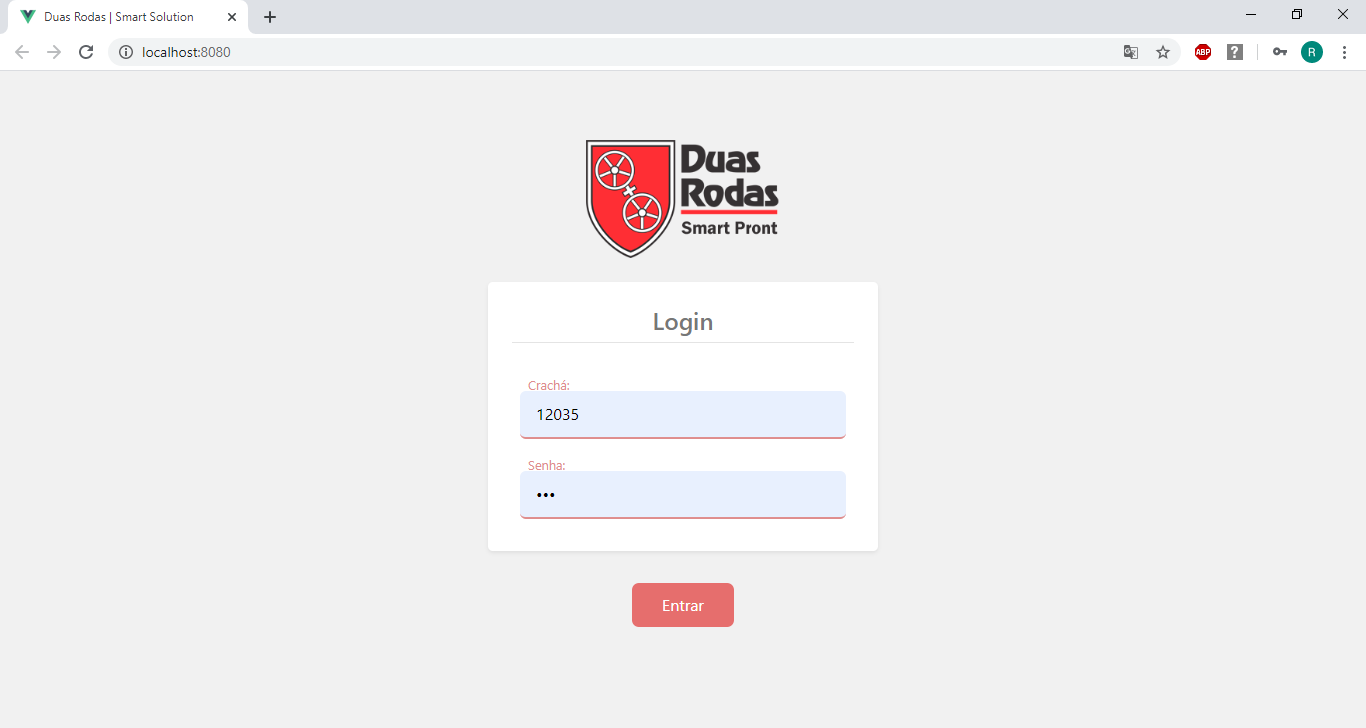
\includegraphics[scale=.55,angle=90]{Figuras/Login_WEB_1}}\qquad
		
	}
	
\end{figure}
\newpage

Tela com as opções de cadastramentos disponíveis no sistema.

\begin{figure}[H]
		\caption{\label{Cadastros_Sistema_1}Tela de opções de cadastros}
	\centering
	\mbox{%
		\subfigure[Próprio autor]{\label{Cadastros_Sistema_1}%
			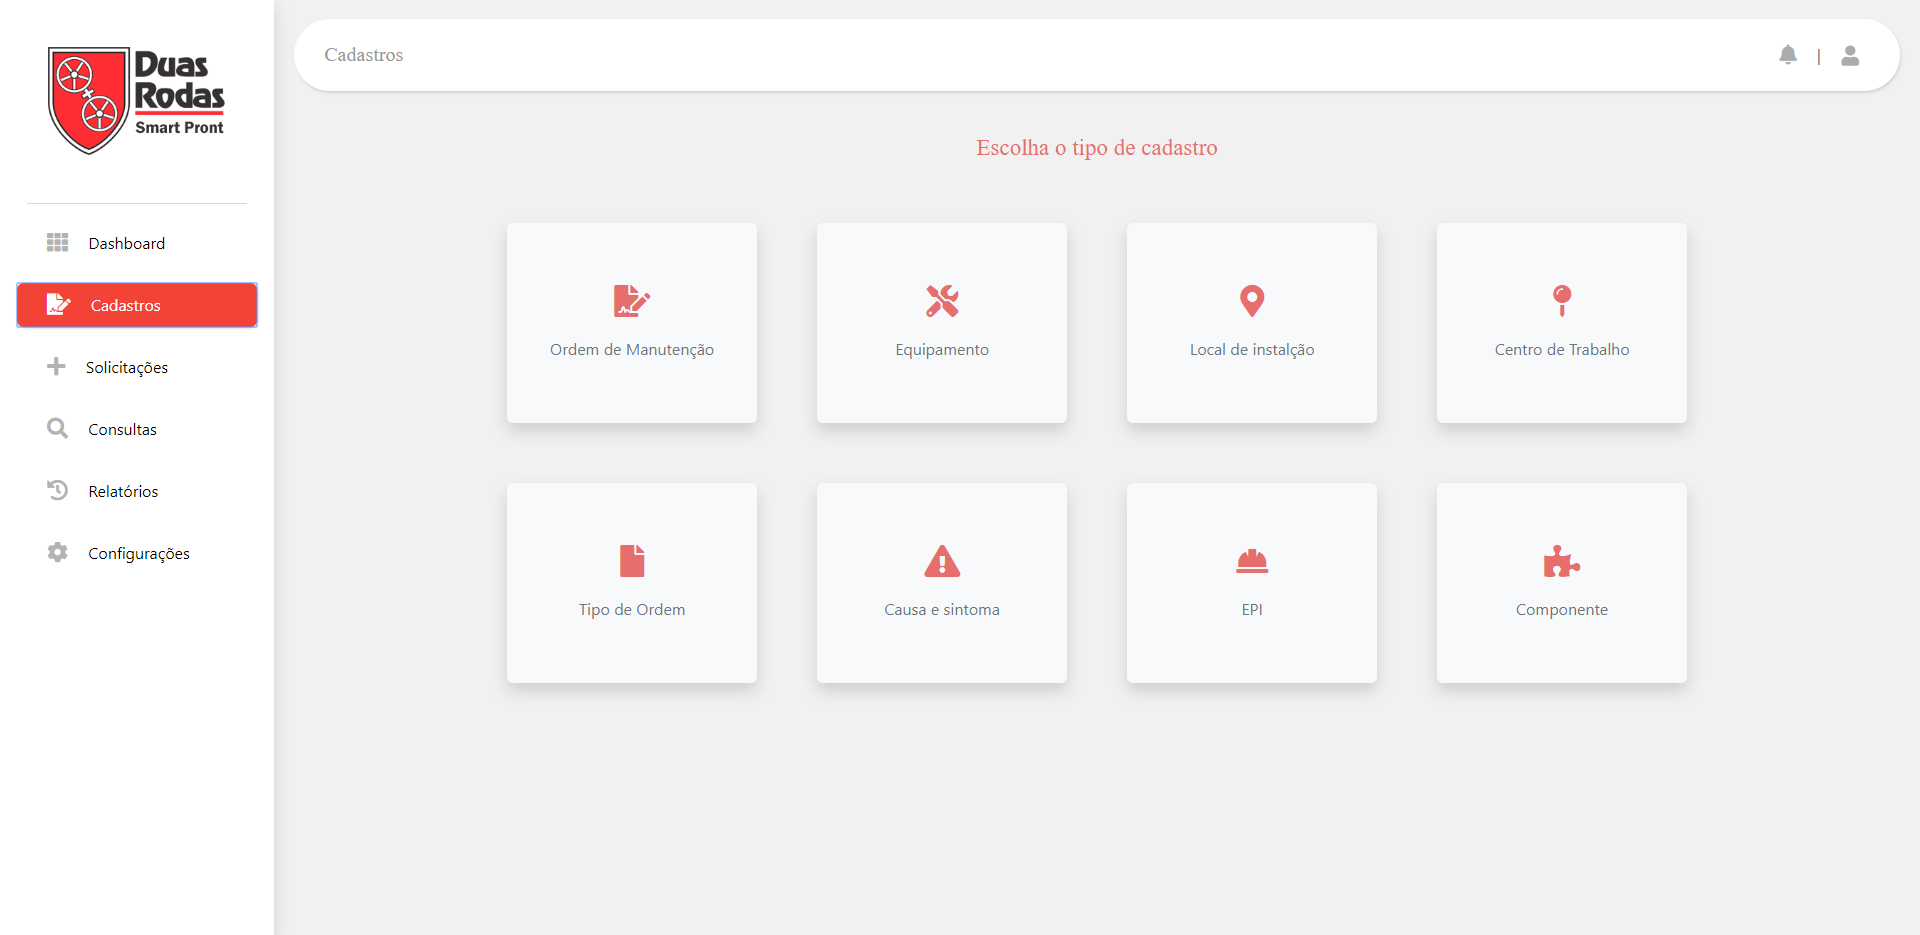
\includegraphics[scale=.45,angle=90]{Figuras/Cadastros_Sistema_1}}\qquad
	}
	
\end{figure}
\newpage

Tela para se cadastrar ordem de serviços no conceito de  step by step no sistema de forma manual primeira etapa.

\begin{figure}[H]
		\caption{\label{step_1}Próprio autor}
	\centering
	\mbox{%
		\subfigure[Tela de cadastro de OS]{\label{step_1}%
			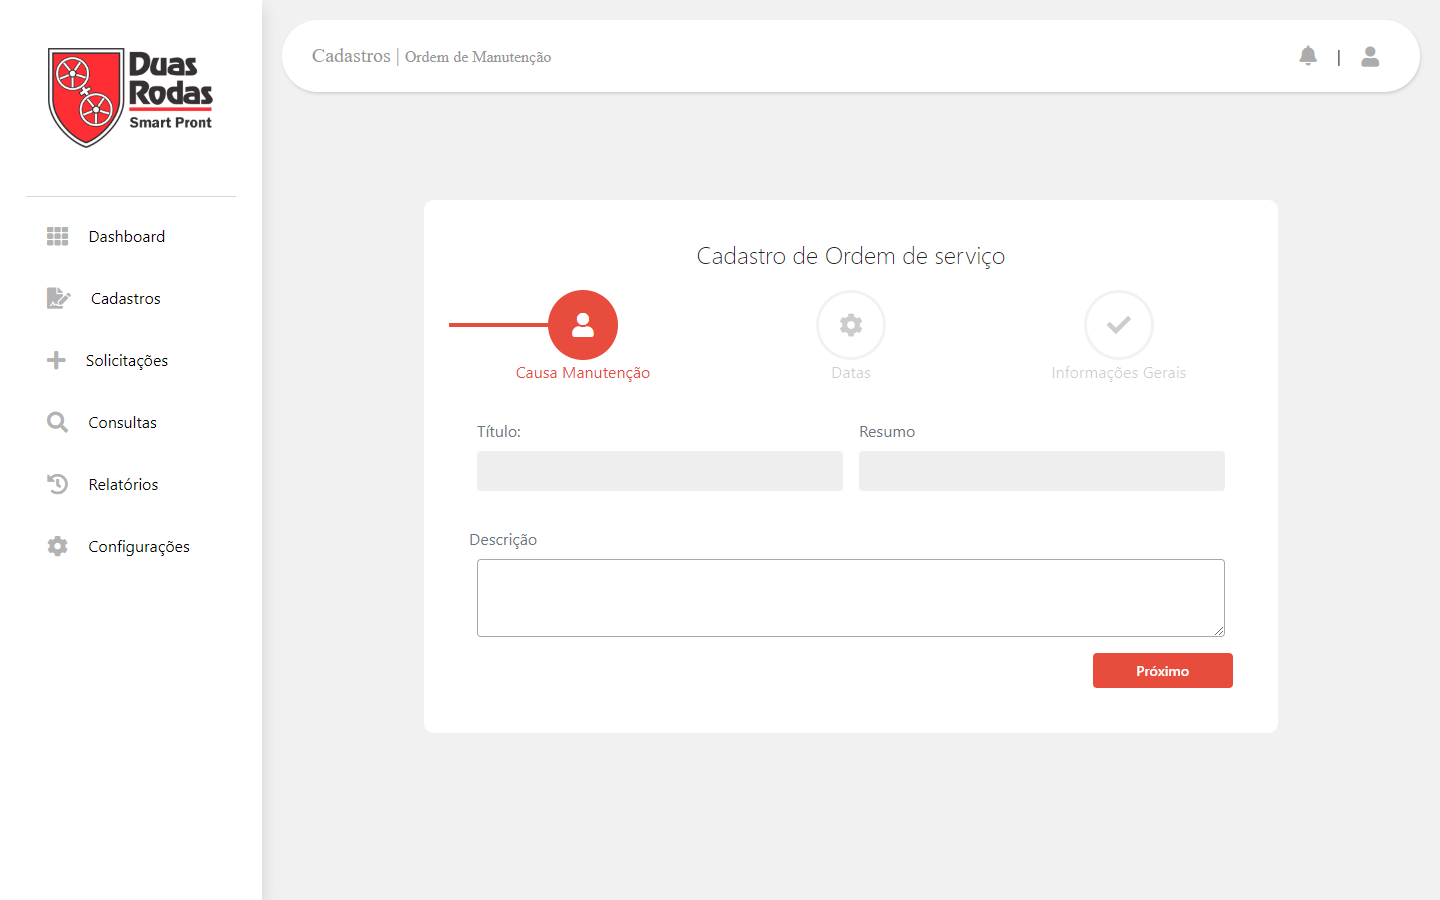
\includegraphics[scale=.42,angle=90]{Figuras/step_1}}\qquad
	}
	
\end{figure}
\newpage

Tela para se cadastrar ordem de serviços no conceito de  step by step no sistema de forma manual segunda etapa

\begin{figure}[H]
		\caption{\label{step_2}Tela de cadastro de OS}
	\centering
	\mbox{%
		\subfigure[Próprio autor]{\label{step_2}%
			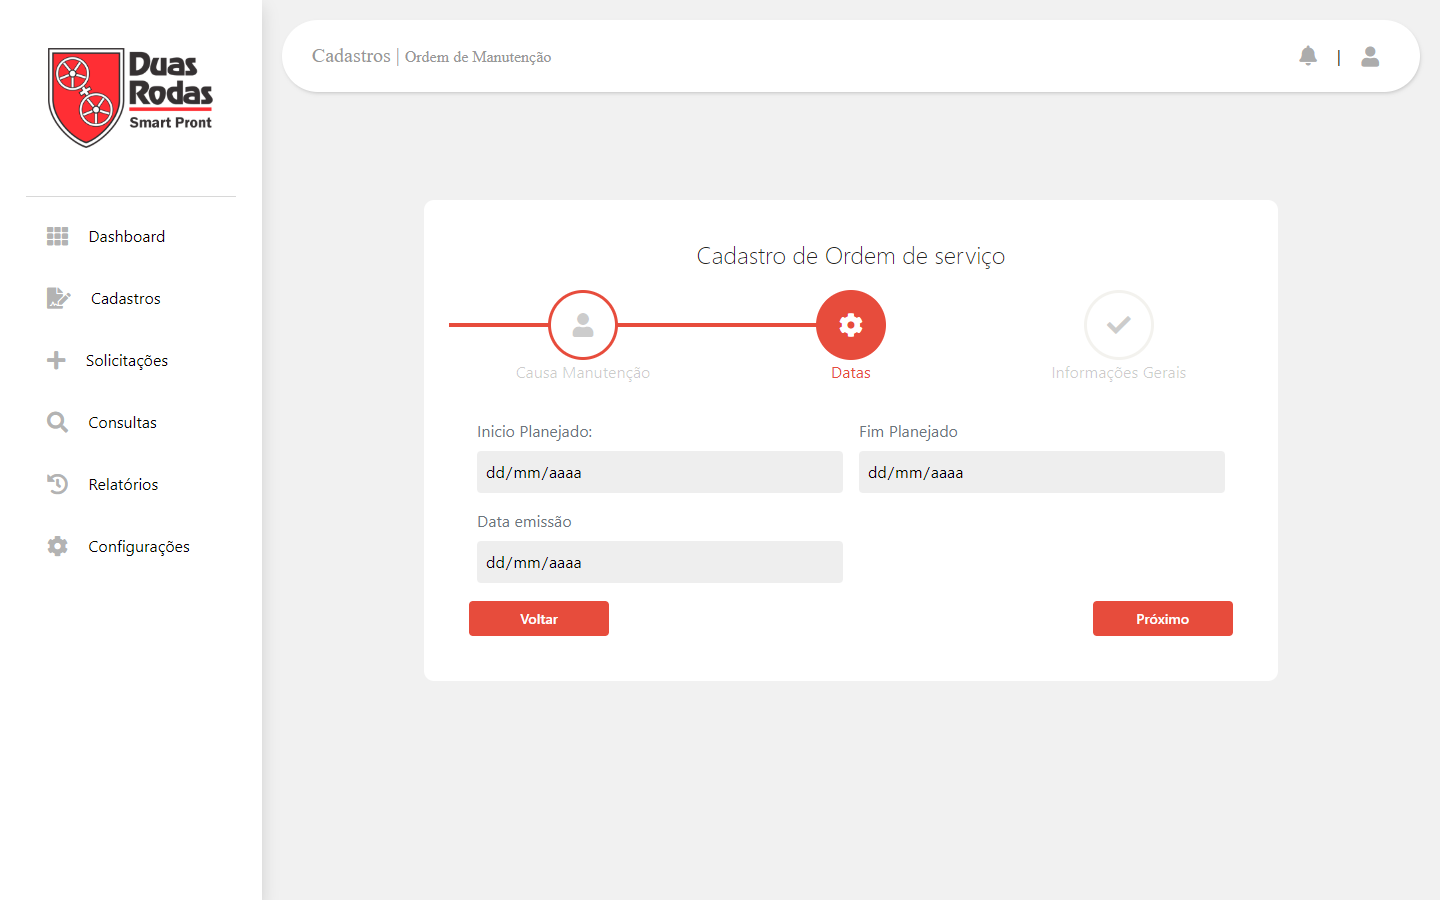
\includegraphics[scale=.42,angle=90]{Figuras/step_2}}\qquad
	}
	
\end{figure}
\newpage

Tela para se cadastrar ordem de serviços no conceito de  step by step no sistema de forma manual terceira etapa

\begin{figure}[H]
		\caption{\label{step_3}Tela de cadastro de OS}
	\centering
	\mbox{%
		\subfigure[Próprio autor]{\label{step_3}%
			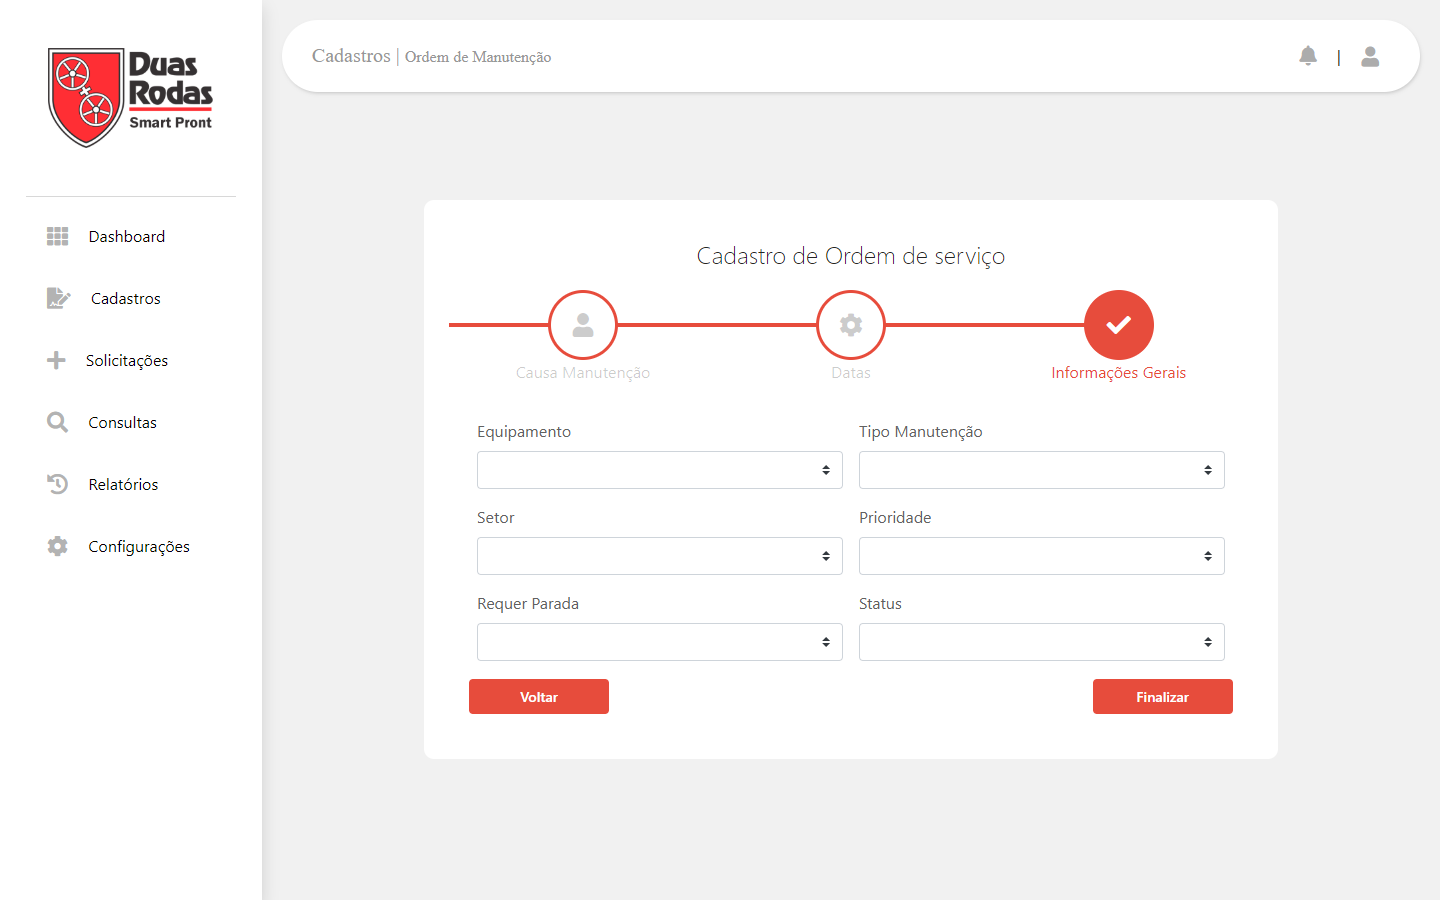
\includegraphics[scale=.42,angle=90]{Figuras/step_3}}\qquad
	}
	
\end{figure}
\newpage

Tela para cadastrar equipamentos no sistema.

\begin{figure}[H]
		\caption{\label{Cadastro_Equipamento_Sistema}Tela de cadastrar equipamentos}
	\centering
	\mbox{%
		\subfigure[Próprio autor]{\label{Cadastro_Equipamento_Sistema}%
			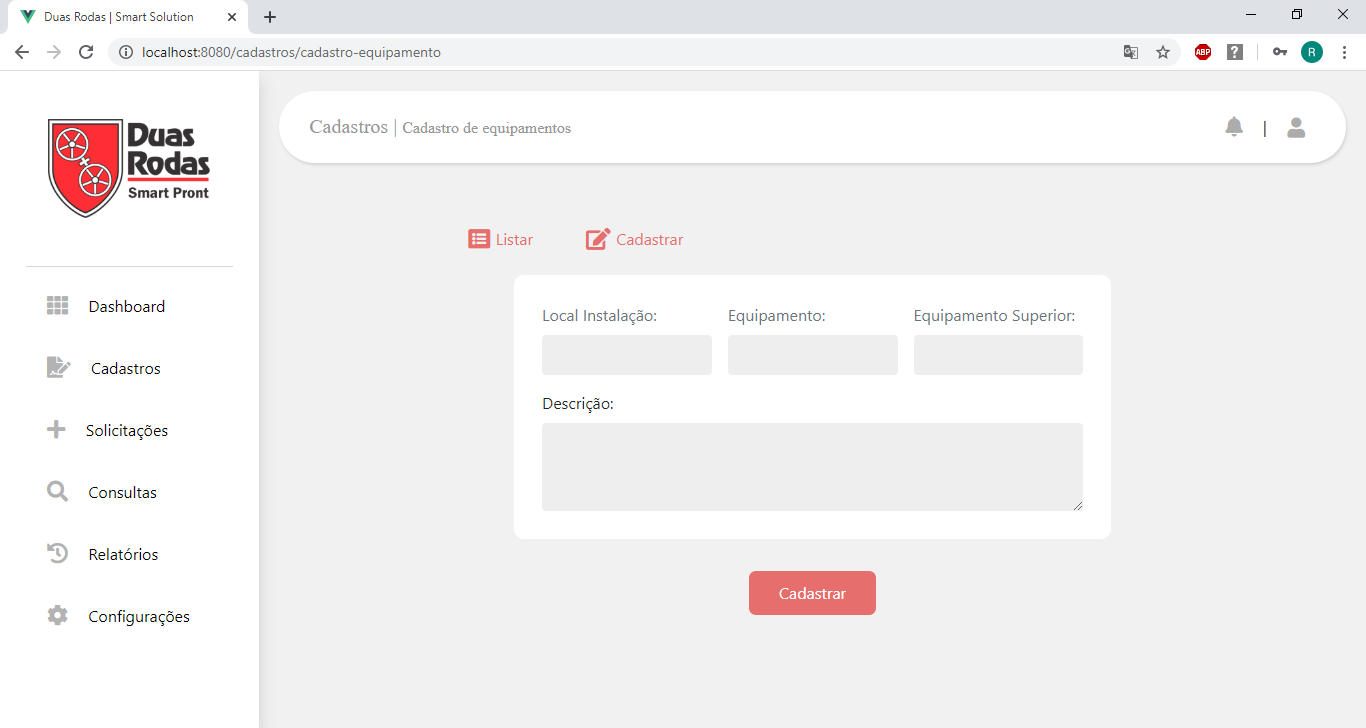
\includegraphics[scale=.62,angle=90]{Figuras/Cadastro_Equipamento_Sistema}}\qquad
	}
	
\end{figure}
\newpage

Tela para cadastrar componentes de cada maquina.

\begin{figure}[H]
		\caption{\label{Cadastro_Componentes} Tela de cadastrar componentes}
	\centering
	\mbox{%
		\subfigure[Próprio autor]{\label{Cadastro_Componentes}%
			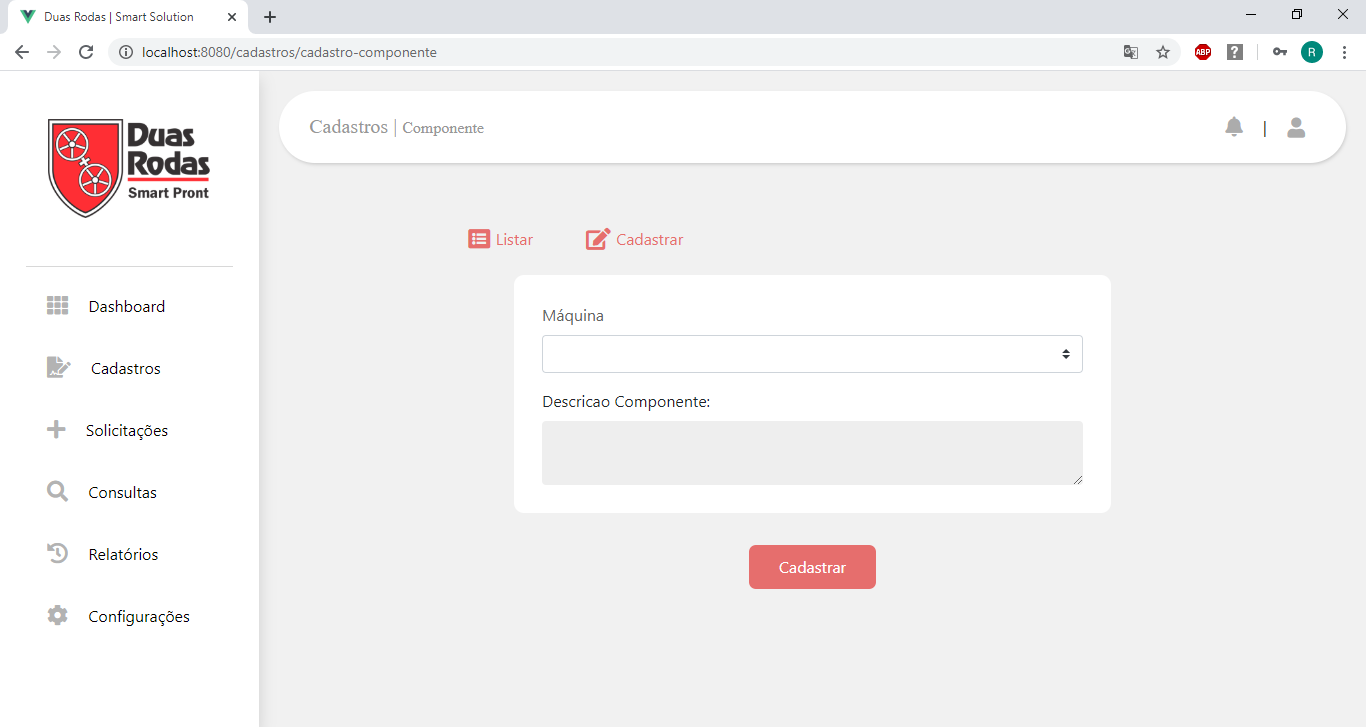
\includegraphics[scale=.62,angle=90]{Figuras/Cadastro_Componentes}}\qquad
	}
	
\end{figure}
\newpage

Tela com finalidade de cadastrar EPI.

\begin{figure}[H]
		\caption{\label{Cadastro_Epi_Sistema} Tela de cadastrar EPI}
	\centering
	\mbox{%
		\subfigure[Próprio autor]{\label{Cadastro_Epi_Sistema}%
			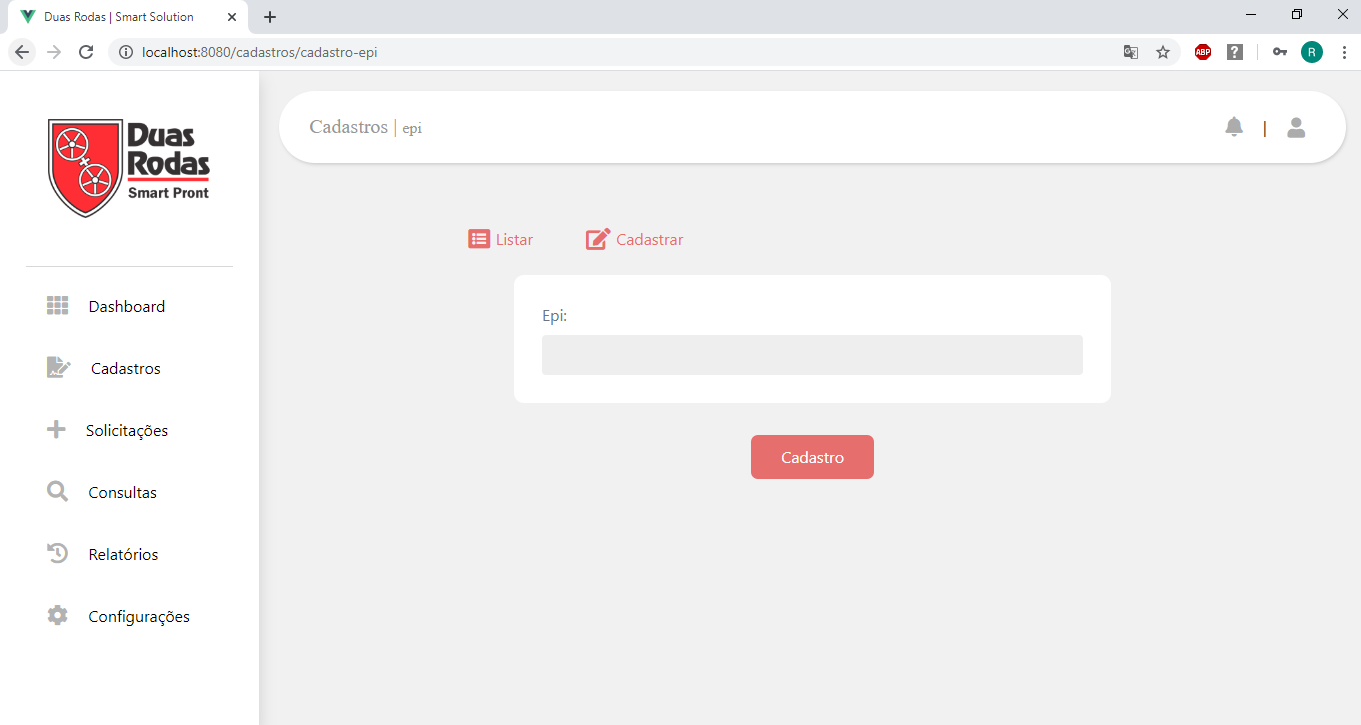
\includegraphics[scale=.62,angle=90]{Figuras/Cadastro_Epi_Sistema}}\qquad
	}
	
\end{figure}
\newpage

Tela para cadastrar causas que ja ocorrerão ou novos.

\begin{figure}[H]
		\caption{\label{Cadastro_Causa_Defeito} Tela de cadastrar causas}
	\centering
	\mbox{%
		\subfigure[Próprio autor]{\label{Cadastro_Causa_Defeito}%
			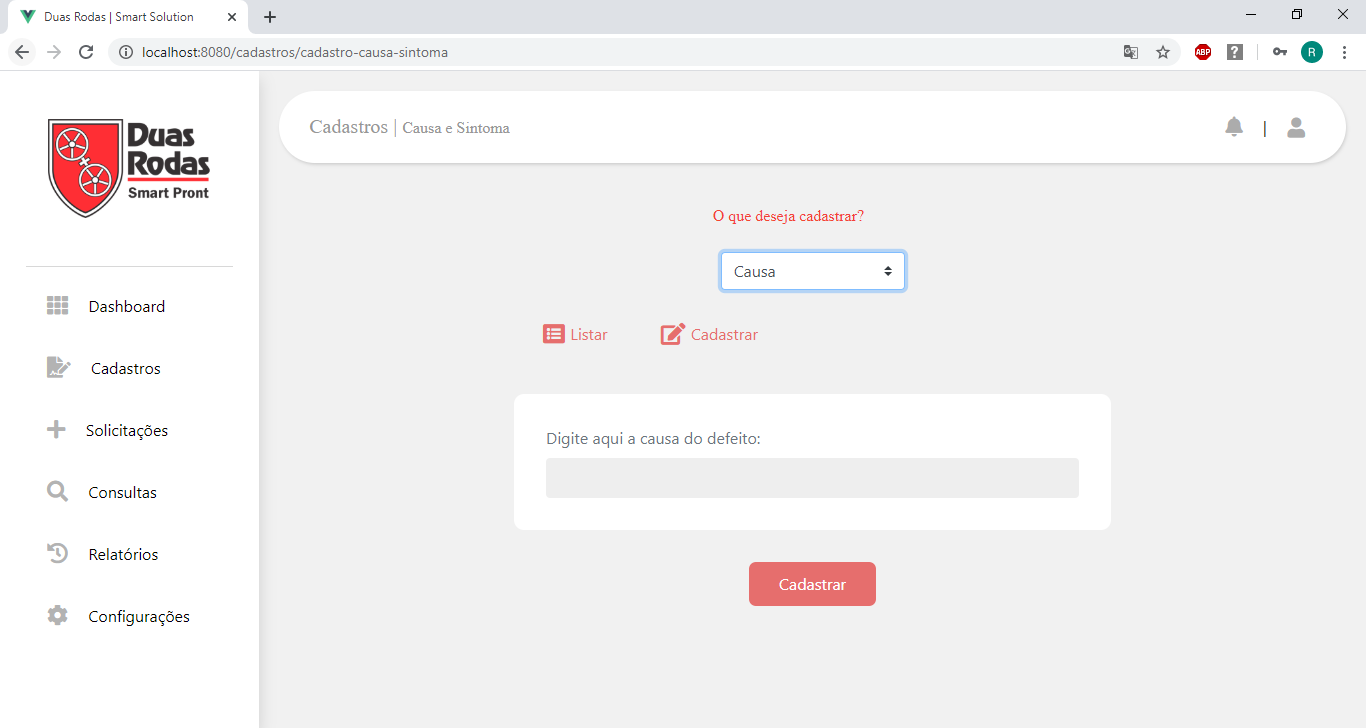
\includegraphics[scale=.62,angle=90]{Figuras/Cadastro_Causa_Defeito}}\qquad
	}
	
\end{figure}
\newpage

Tela para cadastrar sintomas que ja ocorrerão ou novos.

\begin{figure}[H]
		\caption{\label{Cadastro_Sintomas}Tela de cadastrar sintomas}
	\centering
	\mbox{%
		\subfigure[Próprio autor ]{\label{Cadastro_Sintomas}%
			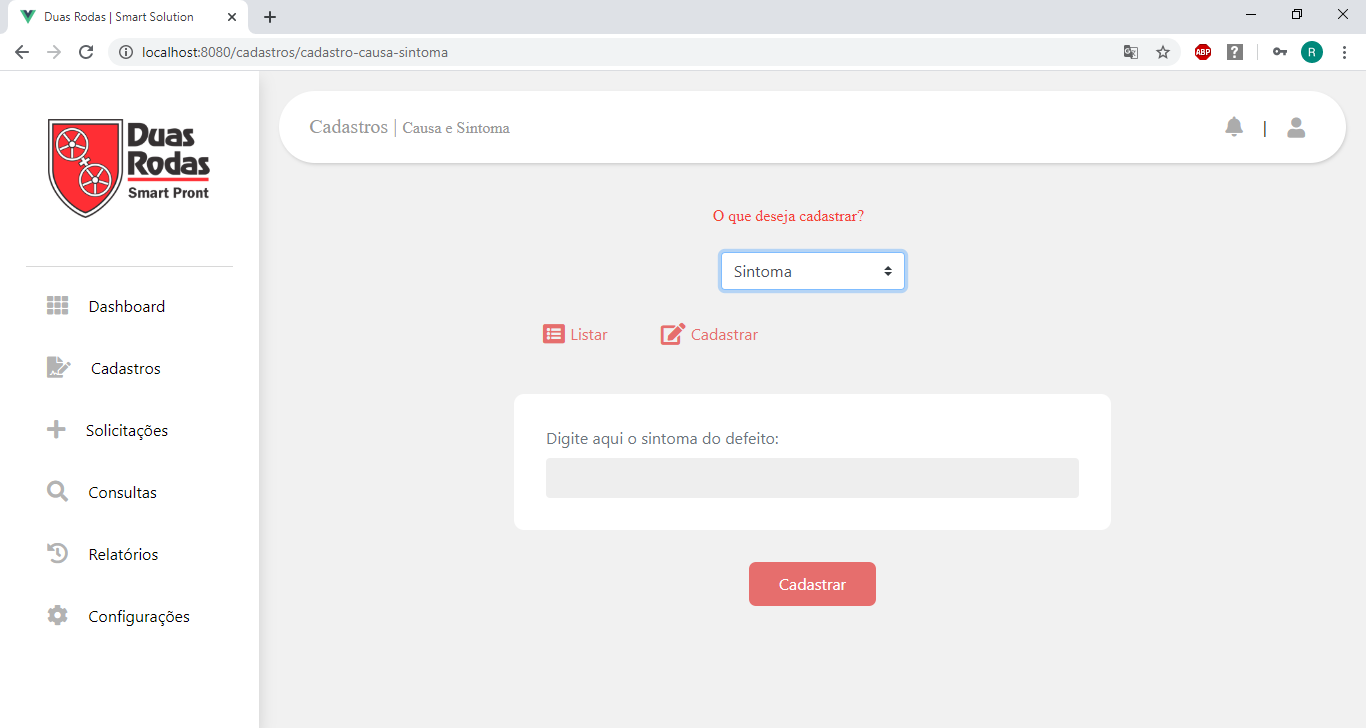
\includegraphics[scale=.62,angle=90]{Figuras/Cadastro_Sintomas}}\qquad
	}
	
\end{figure}
\newpage

Tela para cadastrar localização do equipamento.

\begin{figure}[H]
		\caption{\label{Cadastro_Localizaçao} Tela de cadastrar localização do equipamento}
	\centering
	\mbox{%
		\subfigure[Próprio autor]{\label{Cadastro_Localizaçao}%
			\includegraphics[scale=.62,angle=90]{Figuras/Cadastro_Localizaçao}}\qquad
	}
	
\end{figure}
\newpage


Tela de cadastro de centro de trabalho.

\begin{figure}[H]
		\caption{\label{Cadastro_Centro_Trabalho} Tela de cadastrar centro de trabalho}
	\centering
	\mbox{%
		\subfigure[Próprio autor]{\label{Cadastro_Centro_Trabalho}%
			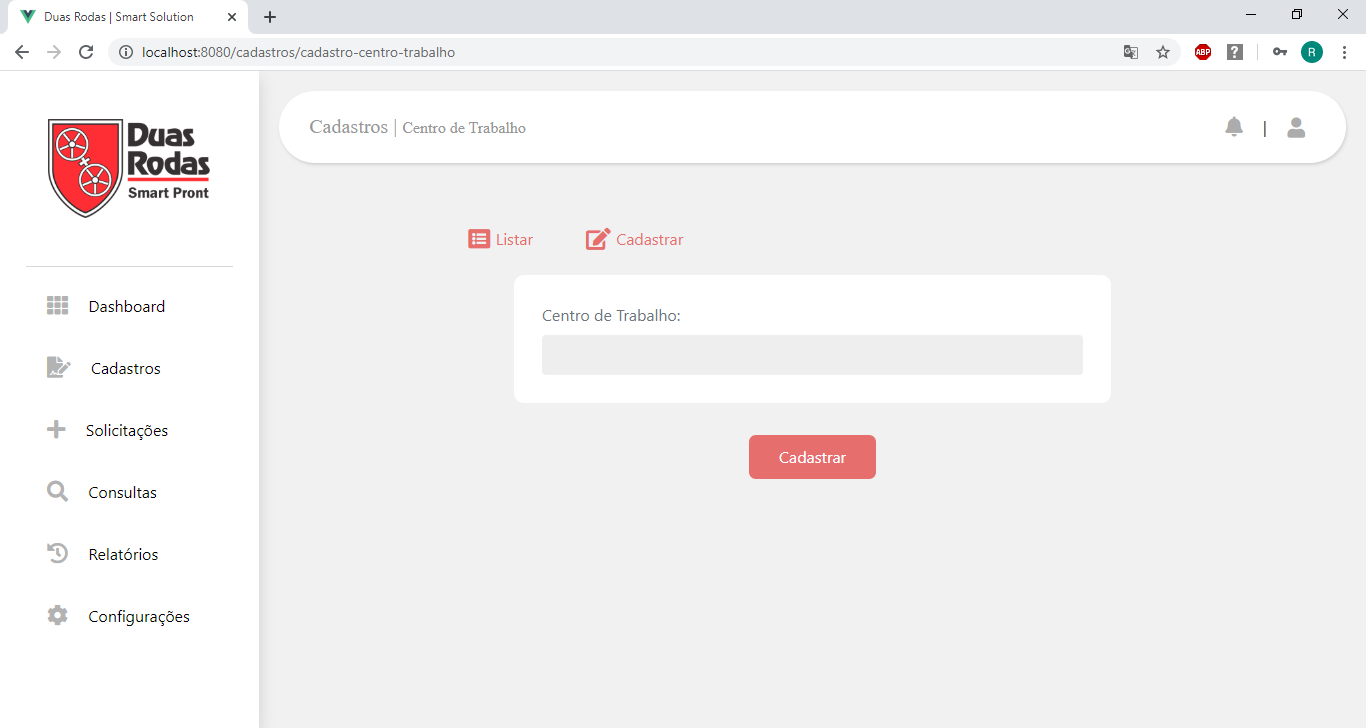
\includegraphics[scale=.62,angle=90]{Figuras/Cadastro_Centro_Trabalho}}\qquad
	}
	
\end{figure}
\newpage

Tela para cadastrar tipo de ordem serviço.

\begin{figure}[H]
		\caption{\label{Cadastro_Tipo_Ordem} Tela de cadastrar tipo de ordem serviço}
	\centering
	\mbox{%
		\subfigure[Próprio autor]{\label{Cadastro_Tipo_Ordem}%
			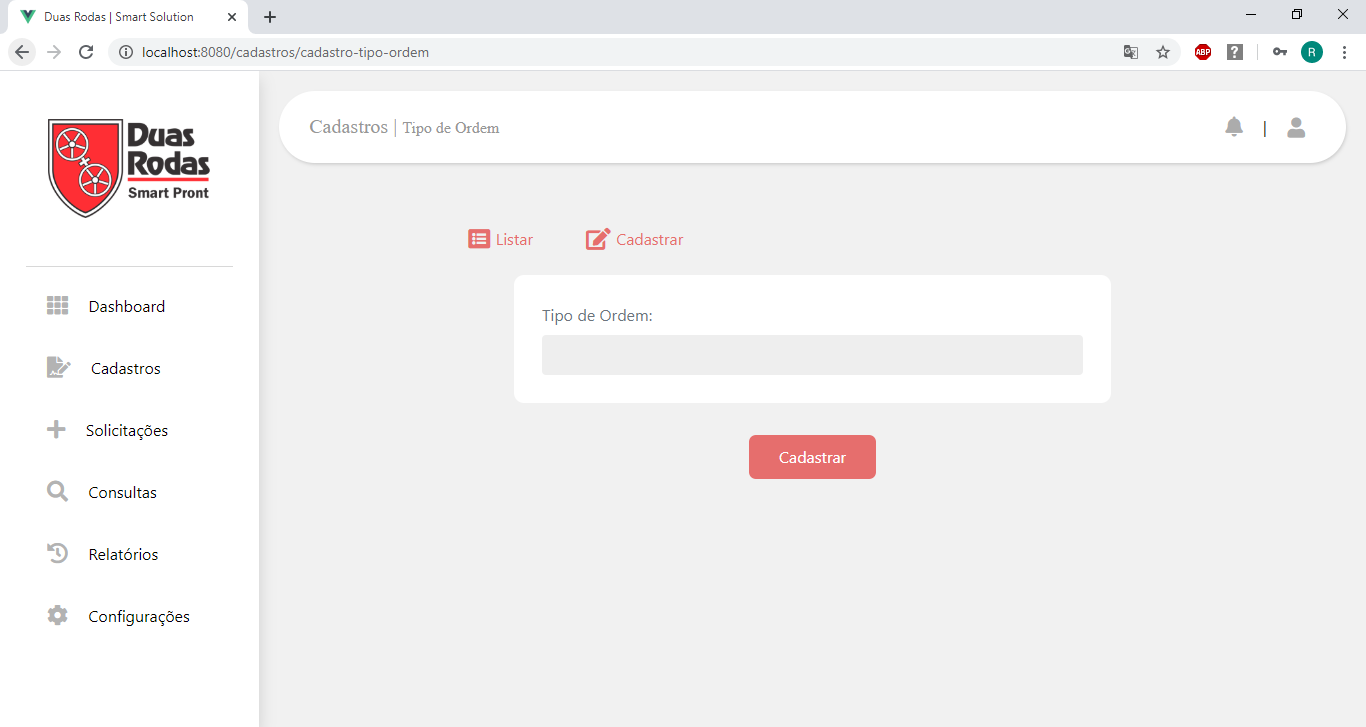
\includegraphics[scale=.62,angle=90]{Figuras/Cadastro_Tipo_Ordem}}\qquad
	}
	
\end{figure}
\newpage


Tela com as opções de cadastrar e listar usuários no sistema.

\begin{figure}[H]
		\caption{\label{listagem_e_cadastro_de_usuario} Tela de cadastrar e listar usuários}
	\centering
	\mbox{%
		\subfigure[Próprio autor]{\label{listagem_e_cadastro_de_usuario}%
			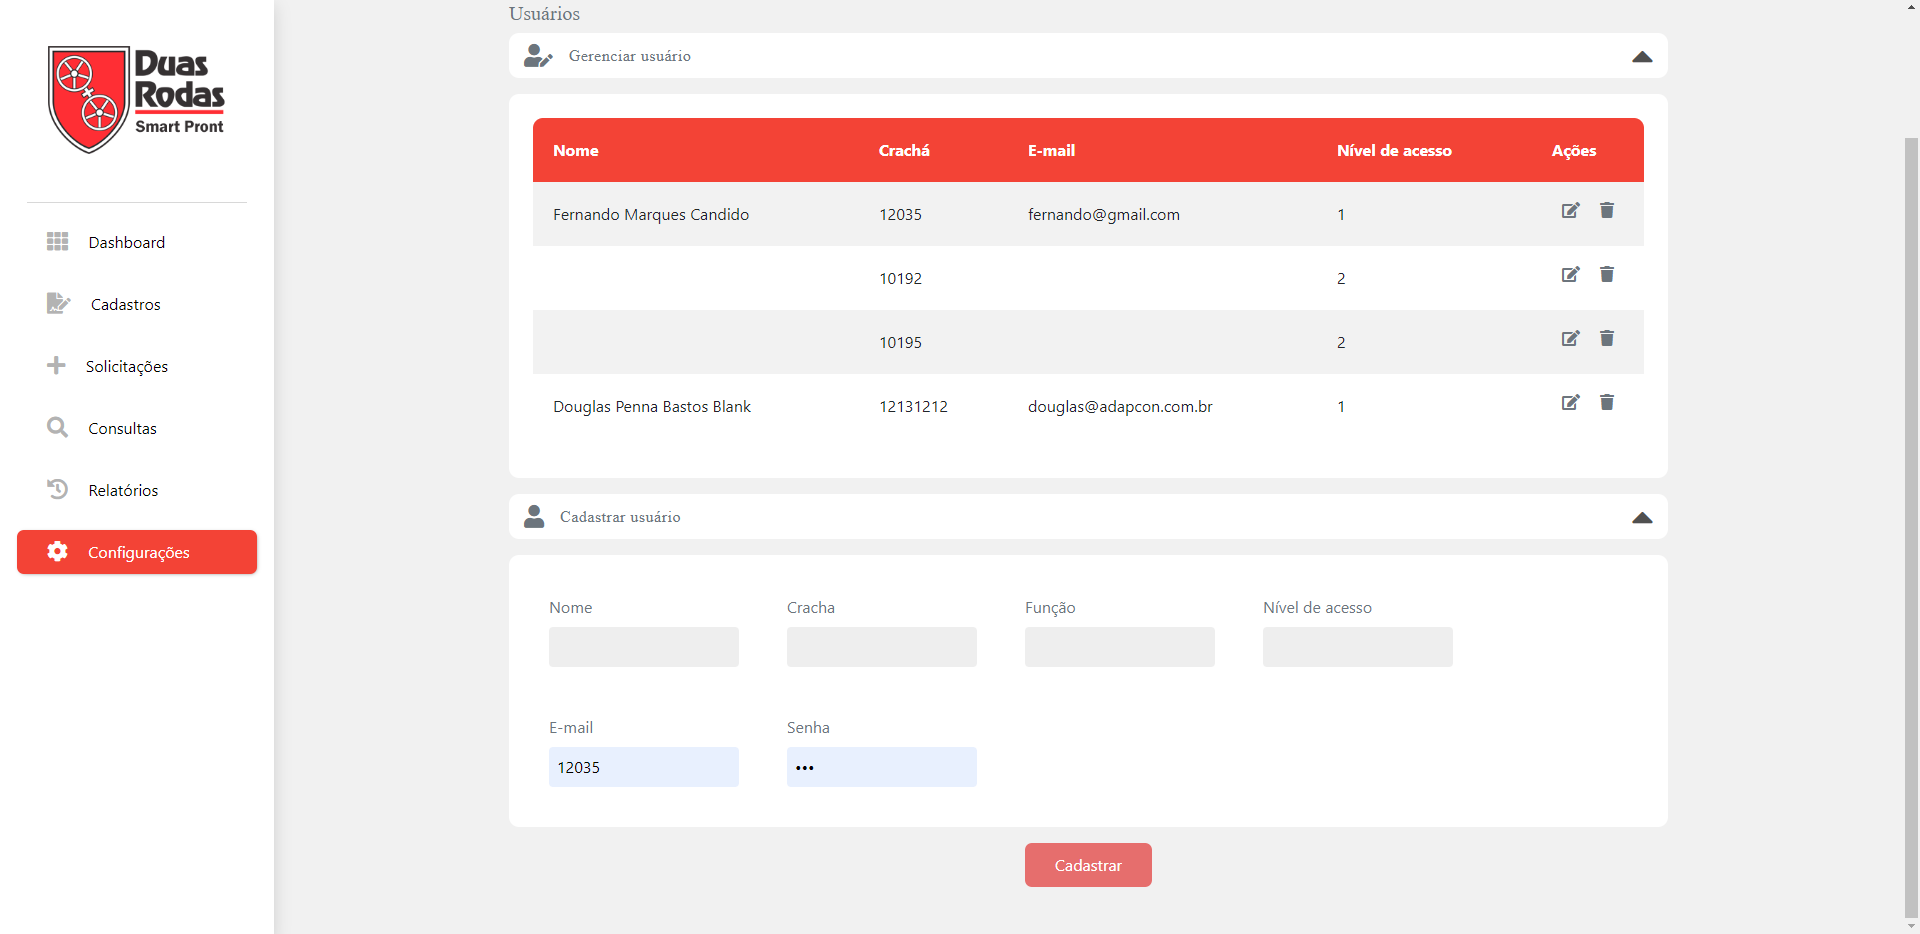
\includegraphics[scale=.47,angle=90]{Figuras/listagem_e_cadastro_de_usuario}}\qquad
	}
	
\end{figure}
\newpage

Tela com as opções de consulta de ordens de serviço no sistema, podendo ser por numero da ordem ou algum dos filtros disponíveis ao usuário.

\begin{figure}[H]
		\caption{\label{Consulta_ordem} Tela de cadastrar e listar usuários}
	\centering
	\mbox{%
		\subfigure[Próprio autor]{\label{Consulta_ordem}%
			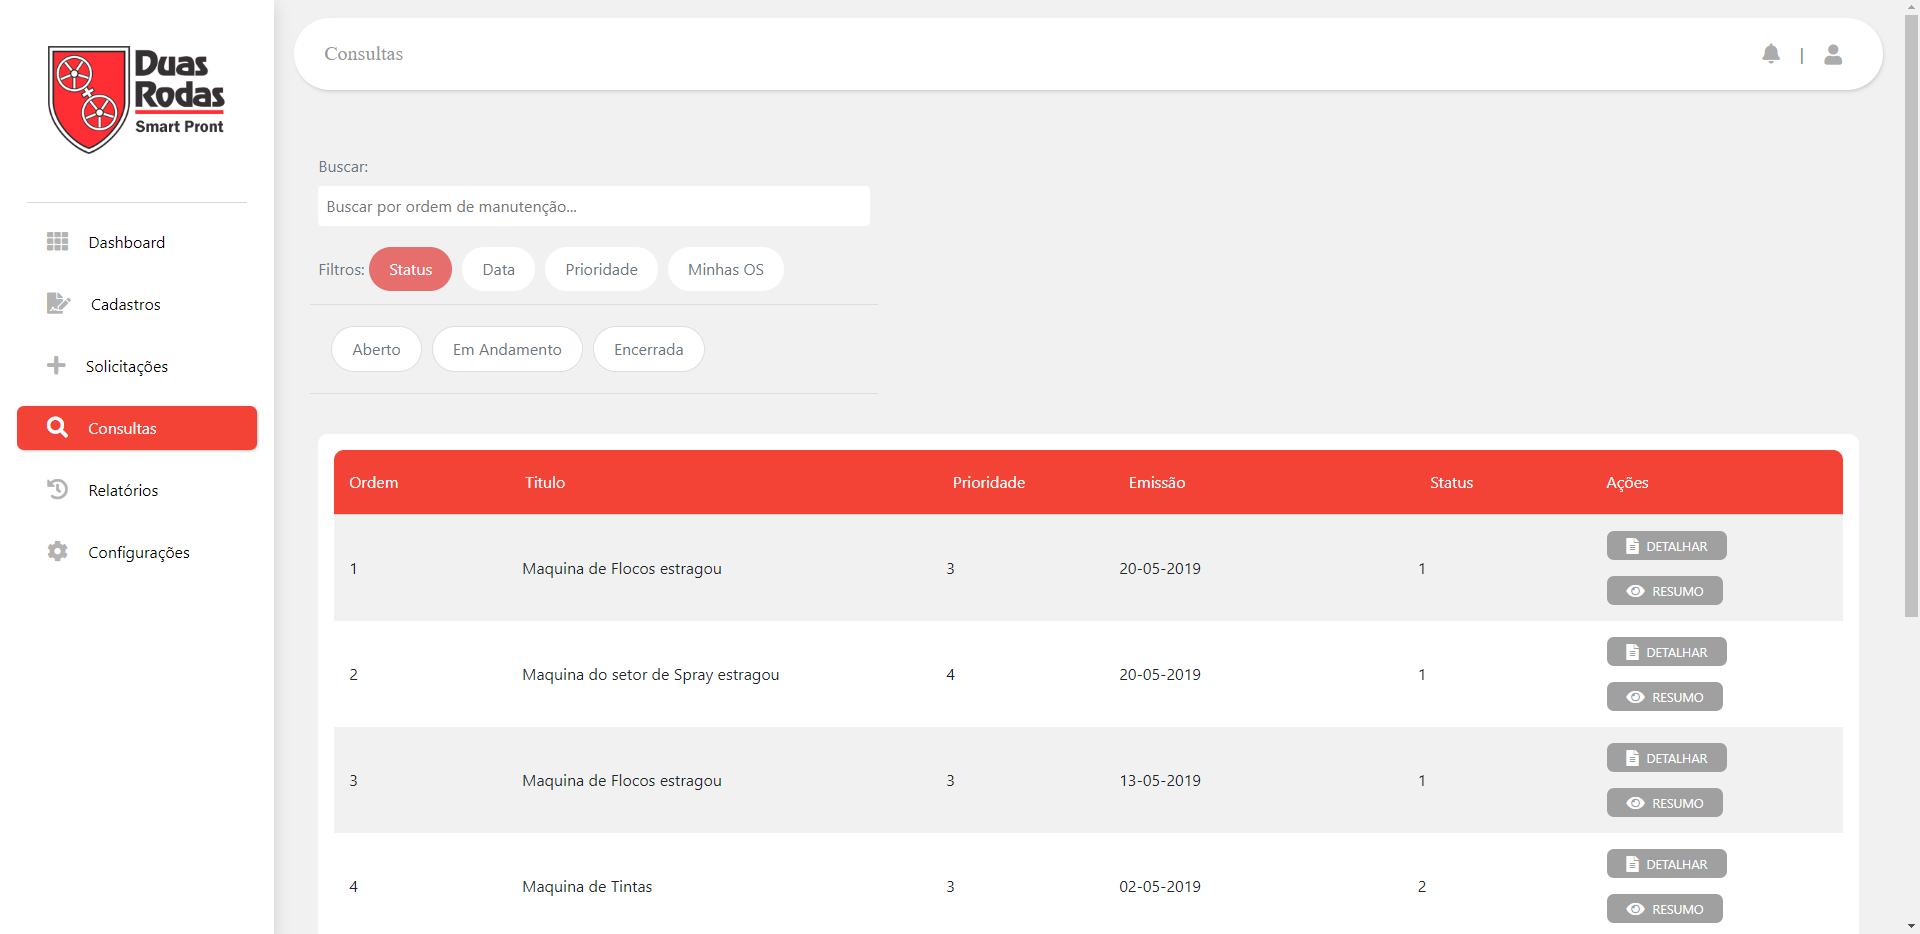
\includegraphics[scale=.45,angle=90]{Figuras/Consulta_ordem}}\qquad
	}
	
\end{figure}
\newpage
% ------